%%%%%%%%%%%%%%%%%%%%%%%%%%%%%%%%%%%%%%%%%%%%%%%%%%%%%%%%%%%%%%%%%%%%%%
% Câu chưa có mã dạng — cần gắn %[..] rồi chuyển vào đúng file dạng
% Số câu: 29  (sinh tự động bởi tach_cau.py; từ nay thầy sửa trực tiếp file này)
%%%%%%%%%%%%%%%%%%%%%%%%%%%%%%%%%%%%%%%%%%%%%%%%%%%%%%%%%%%%%%%%%%%%%%

%%%%%%%%%%%%%%%% TRẢ LỜI NGẮN %%%%%%%%%%%%%%%%

% nguồn: Phan2_Lop_12_Hinh_hoc_Chuong_5
\begin{bt}%[ma:7e001eff]
	%[2H5V1-6] 
	Cho hình  lăng trụ $ABC.A'B'C'$ có $A'ABC$~là tứ diện đều cạnh $a$. Gọi $M$, $N$ lần lượt~là trung điểm của $AA'$ và $BB'$. Tính tang của góc giữa hai mặt phẳng $(ABC)$ và $(CMN)$. Làm tròn kết quả đến hàng phần trăm.
	\shortans{0,57} 
	 \loigiai{
	\immini{Gọi $O$~là trung điểm  của $AB$.\\
		 Chọn hệ trục toạ độ như hình $1$ sao cho $O(0;0;0)$, $A\left(\dfrac{1}{2};0;0\right)$, $B\left(-\dfrac{1}{2};0;0\right)$, $C\left(0;\dfrac{\sqrt{3}}{2};0\right)$, $H\left(0;\dfrac{\sqrt{3}}{6}; 0\right)$.\\
		Vì  $A' H=\dfrac{a \sqrt{6}}{3}$ nên $A'\left(0; \dfrac{\sqrt{3}}{6}; \dfrac{\sqrt{6}}{3}\right)$.\\
		Ta có $\overrightarrow{AB}=\overrightarrow{A' B'} \Rightarrow B'\left(-1; \dfrac{\sqrt{3}}{6}; \dfrac{\sqrt{6}}{3}\right)$.\\ 
		Dễ thấy $(ABC)$  có vectơ pháp tuyến~là $\vec{n}_1=(0; 0; 1)$.\\
		$M$~là trung  điểm $AA'$ $\Rightarrow$ $M\left(\dfrac{1}{4}; \dfrac{\sqrt{3}}{12}; \dfrac{\sqrt{6}}{6}\right)$.\\
		$N$~là trung điểm $BB'$ $\Rightarrow$ $N\left(-\dfrac{3}{4}; \dfrac{\sqrt{3}}{12};  \dfrac{\sqrt{6}}{6}\right)$.\\
		 Do đó $\overrightarrow{MN}=(-1; 0; 0)$, $\overrightarrow{C M}=\left(\dfrac{1}{4};-\dfrac{5 \sqrt{3}}{12}; \dfrac{\sqrt{6}}{6}\right)
		$.}{\resizebox{!}{5cm}{\begin{tikzpicture}[line join=round,line cap=round]
		 \def\a{4}
		 \def\h{4.5}
		\path  (0:0) coordinate (B)
			 ++(0:6/5*\a) coordinate (C)
			++(-150:\a) coordinate (A) 
			($(A)+(82:\h)$) coordinate  (A')
			($(B)+(82:\h)$)  coordinate (B')
			($(C)+(82:\h)$)  coordinate (C')
			($(B)!1/2!(A)$)  coordinate (O)
			($(C)!2/3!(O)$) coordinate (H) 
			($(C)!1/2!(A)$) coordinate (H') 
			 ($(A')!1/2!(A)$) coordinate (M)
			 ($(B)!1/2!(B')$) coordinate (N)
			($(A')+(O)-(H)$) coordinate (z') 
			($(O)!2.3!(z')$) coordinate  (z)
			 ($(O)!5/4!(C)$) coordinate (y)
			($(O)!2!(A)$) coordinate  (x);
		\draw[dashed]  (B)--(C)
			(O)--(C) 
			(B)--(H') 
			(A)--(H)--(A') 
			(C)--(N); 
		 \draw (C)--(C')
			 (B)--(B')
			(A)--(A') 
			 (B)--(A)--(C)
			(A')--(B')--(C')--cycle  (N)--(M)--(C);
		 \draw[-stealth] (A)--(x) node[right]{$x$};
		\draw[-stealth](C)--(y) node[below]{$y$}; 
		\draw[-stealth](O)--(z) node[right]{$z$}; 
		\foreach \x/\g in  {C/-60,B/180,A/-150,A'/-45,B'/45,C'/90,O/-90,H/-70,N/180,M/180}
		 \fill (\x) circle (1pt)
			node[shift={(\g:10pt)}] {$\x$}; 
		\draw  (2/3*\a,-\a) node[above]{\text{ Hình} 1};
	\end{tikzpicture}
		 }}
		\noindent $\Rightarrow(CMN)$  có vectơ pháp tuyến $\vec{n}_2=\left(0; \dfrac{\sqrt{6}}{6}; \dfrac{5\sqrt{3}}{12}\right)=\dfrac{\sqrt{3}}{12}(0; 2\sqrt{2}; 5)$.\\
		Gọi $\varphi$~là góc giữa hai mặt phẳng $(ABC)$ và $(CMN)$, ta  có
		 $$
		\cos \varphi=\dfrac{5}{\sqrt{33}} \Rightarrow \tan \varphi=\sqrt{\dfrac{1}{\cos ^2 \varphi}-1}=\dfrac{2 \sqrt{2}}{5} \approx  0{,}57.
		$$ 
	 }
\end{bt}

% nguồn: Phan2_Lop_12_Hinh_hoc_Chuong_5
\begin{bt}%[ma:32b0fd88]
	%[2H5V2-8] 
	Trong một khung lưới ô vuông gồm các hình lập phương, xét các đường thẳng đi qua hai nút lưới (mỗi nút lưới là đỉnh của hình lập phương), người ta đưa ra một cách kiểm tra độ lệch về phương của hai đường thẳng bằng cách gắn hệ tọa độ $Oxyz$ vào khung lưới ô vuông và tìm vectơ chỉ phương của hai đường  thẳng đó. Giả sử, đường thẳng $a$ đi qua hai nút lưới $M\left(1; 1; 2\right)$ và $N\left(0; 3; 0\right)$, đường thẳng $b$ đi qua hai nút lưới $P\left(1; 0; 3\right)$ và $Q\left(3; 3; 9\right)$. Sau khi làm tròn đến hàng đơn vị của độ thì góc giữa hai đường thẳng $a$ và $b$ bằng $n^\circ$ ($n$ là số tự nhiên). Giá trị của $n$ bằng bao~nhiêu?
	 \shortans{68}
	\loigiai{ 
		Vectơ chỉ phương của đường  thẳng $a$ là $\overrightarrow{u} = \overrightarrow{MN} = \left(0-1; 3-1; 0-2\right) = \left(-1; 2; -2\right)$.\\
		Vectơ chỉ phương của đường thẳng $b$ là $\overrightarrow{v} = \overrightarrow{PQ} = \left(3-1; 3-0; 9-3\right)  = \left(2; 3; 6\right)$.\\
		Gọi $\theta$ là góc giữa hai đường thẳng $a$  và $b$. \\
		 Ta có
		$$\cos \theta = \dfrac{|\overrightarrow{u} \cdot \overrightarrow{v}|}{|\overrightarrow{u}| |\overrightarrow{v}|} =\dfrac{\left|-1 \cdot 2 + 2 \cdot 3 - 2 \cdot 6 \right|}{\sqrt{1 + 4 +  4}\cdot \sqrt{4 + 9 + 36}} =\dfrac{8}{21}.$$
		Suy ra $\theta \approx  67{,}606^\circ$.\\
		Làm tròn đến hàng đơn vị của  độ, ta được $n = 68$. \\
		Vậy giá trị của $n$  là $68$.
	} 
\end{bt}

% nguồn: Phan2_Lop_12_Hinh_hoc_Chuong_5
\begin{bt}%[ma:33b631a4]
	%[2H5H1-3] 
	Trong không gian $Oxyz$, mặt phẳng $\left(\alpha\right)$ đi qua điểm $M(5;4;3)$ và cắt các tia $Ox$, $Oy$, $Oz$ các đoạn bằng nhau có phương  trình~là $x+ay+bz+c=0$. Tìm giá trị của $c$.
	\shortans{-12} 
	\loigiai{ 
		Gọi $A(m;0;0)$, $B(0;m;0)$, $C(0;0;m)$ với $m>0$~là giao điểm của mặt phẳng  $\left(\alpha\right)$ và các tia $Ox$, $Oy$, $Oz$.\\
		Phương trình mặt phẳng $\left(\alpha\right)$ đi qua $A$,  $B$, $C$~là $\dfrac{x}{m}+\dfrac{y}{m}+\dfrac{z}{m}=1$.\\
		Mặt phẳng $\left(\alpha\right)$ qua điểm $M(5;4;3)$, suy  ra $m=12$.\\
		Ta  có $\dfrac{x}{12}+\dfrac{y}{12}+\dfrac{z}{12}=1 \Leftrightarrow x+y+z-12=0$. Suy ra $c=-12$.
	} 
\end{bt}

% nguồn: Phan2_Lop_12_Hinh_hoc_Chuong_5
\begin{bt}%[ma:f693121c]
	 %[2H5C2-7]
	Cho hình chóp tứ giác đều $S.ABCD$ có đáy $ABCD$~là hình vuông cạnh $a$. Gọi $O$~là giao điểm của $AC$ và $BD$; $M$ và $N$ lần lượt~là trung điểm của hai cạnh $SA$ và $BC$. Biết $MN=\dfrac{a \sqrt{6}}{2}$. Tính sin của góc  giữa đường thẳng $MN$ và mặt phẳng ($SBD$). Làm tròn kết quả đến hàng phần trăm.
	 \shortans{0,58}
	 \loigiai{
	\immini{Gọi $I$ hình chiếu của  $M$ lên ($ABCD$), suy ra $I$~là trung điểm của $AO$.\\
		Khi đó $CI=\dfrac{3}{4}  AC=\dfrac{3a \sqrt{2}}{4}$.\\
		Xét $\triangle CNI$  có $CN=\dfrac{a}{2}$, $\widehat{NCI}=45^{\circ}$.\\
		Áp  dụng định lí côsin, ta có
		$$ 
		\begin{aligned}
			N I &=\sqrt{C N^2+C I^2-2 C N \cdot C  I \cdot \cos 45^{\circ}} \\
			&=\sqrt{\dfrac{a^2}{4}+\dfrac{9 a^2}{8}-2 \cdot \dfrac{a}{2} \cdot \dfrac{3 a \sqrt{2}}{4} \cdot \dfrac{\sqrt{2}}{2}}=\dfrac{a \sqrt{10}}{4}. 
		\end{aligned}
		 $$
		Xét $\triangle MIN$ vuông tại $I$ nên 
		 $$
		M  I=\sqrt{MN^2-N I^2}=\sqrt{\dfrac{3 a^2}{2}-\dfrac{5 a^2}{8}}=\dfrac{a \sqrt{14}}{4}.
		 $$
		Mà $MI\parallel SO$, $MI=\dfrac{1}{2} SO$ $\Rightarrow$ $SO=\dfrac{a \sqrt{14}}{2}$.}{\begin{tikzpicture}[font=\footnotesize,line join=round,line cap=round]
		\def\a{4} 
		\path (0:0) coordinate (A) 
			++(0:\a) coordinate (B) 
			++(-130:\a/2)  coordinate (C)
			($(A)+(C)-(B)$)  coordinate (D)
			 ($(A)+(70:\a)$) coordinate (S)
			(intersection of A--C and B--D) coordinate (O) 
			 ($(A)!1/2!(O)$) coordinate (I)
			 ($(A)!1/2!(S)$) coordinate (M)
			($(B)!1/2!(C)$)  coordinate (N)
			($(O)!2!(C)$)  coordinate (x)
			 ($(O)!3/2!(B)$) coordinate (y)
			($(O)!4/3!(S)$)  coordinate (z);
		\draw[dashed]  (B)--(A)--(D)
			 (A)--(S)--(O)
			(A)--(C) 
			(B)--(D) 
			 (I)--(M)--(N)--(I);
		\draw (B)-- (C)--(D) 
			(B)--(S) 
			 (C)--(S)
			(D)--(S); 
		\draw[-stealth] (C)--(x) node[above]{$x$}; 
		 \draw[-stealth](B)--(y) node[below]{$y$};
		\draw[-stealth](S)--(z) node[right]{$z$}; 
		\foreach \x/\g in {A/135,D/-135,C/-90,B/60,S/180,O/-90,M/10,I/-100,N/-30} 
		\fill (\x)  circle (1pt)
			node[shift={(\g:10pt)}]  {$\x$};
		\draw (\a/2.3,-2/3*\a)  node[above]{\text{ Hình} $2$};
	\end{tikzpicture}
		} 
		\noindent Chọn  hệ trục toạ độ $Oxyz$ như Hình $2$.\\
		Ta có $O(0; 0; 0)$, $B\left(0; \dfrac{\sqrt{2}}{2}; 0\right)$, $D\left(0;-\dfrac{\sqrt{2}}{2}; 0\right)$, $C\left(\dfrac{\sqrt{2}}{2}; 0; 0\right)$, $N\left(\dfrac{\sqrt{2}}{4};  \dfrac{\sqrt{2}}{4}; 0\right)$, $A\left(-\dfrac{\sqrt{2}}{2}; 0; 0\right)$, $S\left(0; 0; \dfrac{\sqrt{14}}{2}\right)$, $M\left(-\dfrac{\sqrt{2}}{4}; 0; \dfrac{\sqrt{14}}{4}\right)$.\\
		Khi đó $\overrightarrow{MN}=\left(\dfrac{\sqrt{2}}{2}; \dfrac{\sqrt{2}}{4};-\dfrac{\sqrt{14}}{4}\right)$,  $\overrightarrow{SB}=\left(0; \dfrac{\sqrt{2}}{2};-\dfrac{\sqrt{14}}{2}\right)$, $\overrightarrow{SD}=\left(0;-\dfrac{\sqrt{2}}{2};-\dfrac{\sqrt{14}}{2}\right)$.\\
		Vectơ pháp tuyến  của mặt phẳng $(SBD)\colon \vec{n}=\overrightarrow{SB} \wedge \overrightarrow{SD}=(-\sqrt{7}; 0; 0)$.\\
		Suy ra $\sin (MN,(SBD.)=\dfrac{|\overrightarrow{MN} \cdot \vec{n}|}{|\overrightarrow{MN}|\cdot|\vec{n}|}=\dfrac{\left|\dfrac{\sqrt{2}}{2} \cdot(-\sqrt{7})\right|}{\dfrac{\sqrt{6}}{2} \cdot \sqrt{7}}=\dfrac{\sqrt{3}}{3} \approx  0{,}58$.
	} 
\end{bt}

% nguồn: Phan2_Lop_12_Hinh_hoc_Chuong_5
\begin{bt}%[ma:5b79003e]
	 %[2H5V2-8]
	Trong không gian $Oxyz$, đài kiểm soát không lưu sân bay có tọa độ $O(0;0;0)$, đơn vị trên mỗi trục tính theo kilômét. Một máy bay chuyển động hướng về đài kiểm soát không lưu, bay qua hai vị trí $A(-500;-250;150)$, $B(-200;-200;100)$. Khi máy bay ở gần  đài kiểm soát nhất, tọa độ của vị trí máy bay là $(a;b;c)$. Giá trị của biểu thức $-3a-b-c$ là bao~nhiêu (làm tròn kết quả đến hàng đơn vị)?
	 \shortans{3150}
	\loigiai{ 
		Véc-tơ $\overrightarrow{AB}=(300;50;-50)$ nên $\overrightarrow{u}=(6;1;-1)$ là một véc-tơ chỉ phương của đường thẳng $AB$.\\ Phương  trình đường thẳng $AB$ là
		$$\dfrac {x+500}{6}=\dfrac {y+250}{1}=\dfrac  {z-150}{-1}.$$
		Gọi $H$ là hình chiếu của  điểm $O$ trên đường thẳng $AB$ thì $OH$ là khoảng cách ngắn nhất giữa máy bay và đài kiểm soát. Khi đó $H(6t-500;t-250;-t+150)$.\\
		Ta có $\overrightarrow{OH}\cdot \overrightarrow{u}=(6t-500)\cdot  6+t-250+(-t+150)=0\Leftrightarrow t=-\dfrac {775}{9}$.\\
		Suy ra toạ độ của vị trí  máy bay khi đó là $\left( -\dfrac {3\,050}{3};-\dfrac {3\,025}{9};\dfrac {2\,125}{9} \right)$.\\
		Vậy $-3a-b-c=3\,150$. 
	} 
\end{bt}

% nguồn: Phan2_Lop_12_Hinh_hoc_Chuong_5
\begin{bt}%[ma:7de77b5c]
	%[2H5C3-4] 
	Trong khối pha lê hình lập phương $ABCD.A'B'C'D'$ cạnh $8$ (cm) có mặt cầu cách đều các mặt của hình lập phương $ABCD.A'B'C'D'$ một khoảng $1$ (cm). Chọn hệ trục tọa~độ $Oxyz$  sao cho đỉnh $A$ trùng với gốc tọa~độ $O$, đỉnh $B$ thuộc tia $Ox$, đỉnh $D$ thuộc tia $Oy$, đỉnh $A'$ thuộc tia $Oz$. Khi đó, phương trình của mặt cầu bên trong khối pha lê hình lập phương~là $x^2 +y^2 +z^2+2ax+2by+2cz+d=0$. Tìm giá trị của $a+b+c+d$.
	\shortans{51} 
	\loigiai{ 
	\immini{ 
		Gọi $I$~là  tâm của hình lập phương.\\
		Khối pha lê hình lập phương $ABCD.A'B'C'D'$ cạnh  $8$ (cm).\\
		Chọn hệ trục tọa~độ $Oxyz$ sao cho đỉnh $A$ trùng với gốc tọa~độ $O$, đỉnh $B$ thuộc tia $Ox$, đỉnh $D$ thuộc tia $Oy$, đỉnh $A'$ thuộc tia $Oz$. Khi  đó, tọa~độ các đỉnh của hình lập phương~là
		\begin{eqnarray*}
			& & A(0;0;0), B(8;0;0),  C(8;8;0), D(0;8;0), \\
			&  & A'(0;0;8), B'(8;0;8), C'(8;8;8), D'(0;8;8).
		\end{eqnarray*}
		} 
		{ 
		\begin{tikzpicture}[scale=0.7,font=\scriptsize,>=stealth]
				\def\a{4} 
				\path 
					(0:0) coordinate  (A)
					 (-15:\a) coordinate (B)
					(25:0.8*\a)  coordinate (D)
					($(B)+(D)-(A)$) coordinate  (C)
				\foreach \x in {A,B,C,D}{(\x)++(90:\a) coordinate  (\x')}
					($(A)!0.5!(C')$) coordinate (I) 
					 ($(A)!0.5!(D')$) coordinate (M)
					($(A)!1.3!(B)$)  coordinate (x)
					($(A)!1.6!(D)$) coordinate  (y)
					($(A)!1.3!(A')$)  coordinate (z);
				 \draw (A')--(B')--(B)--(A)--cycle (B)--(C)--(C')--(B')
					(A')--(D')--(C'); 
				\draw[dashed]  (A)--(D)--(C)
					(D)--(D') 
					(I)--(M); 
				\draw[-stealth] (B)--(x)  node[above] {$x$};
				\draw[-stealth,dashed] (D)--(y) node[above] {$y$}; 
				 \draw[-stealth] (A')--(z) node[right] {$z$};
				\foreach \x/\g  in {A/180,B/-90,C/0,D/150,A'/180,B'/90,C'/0,D'/90,I/90,M/90}
				\draw (\x) circle  (0.02) +(\g:0.3) node{\x};
				\node[below] (A) {$O$}; 
			\end{tikzpicture}
		} 
		 \vspace*{10pt}
		\noindent Suy ra tọa~độ tâm  $I$~là $I(4;4;4)$.\\
		 Ta có: $\mathrm{d}(I,(BCC'B')) = IM = \dfrac{1}{2} AB = \dfrac{1}{2} \cdot 8 = 4$ (cm).\\
		Do trong khối pha lê hình lập phương $ABCD.A'B'C'D'$ có mặt cầu cách đều các mặt của hình lập phương một khoảng $1$ (cm) nên tâm $I$ của hình lập phương  chính~là tâm của mặt cầu và bán kính mặt cầu bằng
		$$R= \mathrm{d}(I,(BCC'B')) -1 = 4 -1= 3 \text{ (cm)}.$$ 
		Mặt cầu có tâm~là $I(4;;4;4)$, bán kính $R=3$ nên có phương  trình~là\\
		$(x-4)^2 +(y-4)^2 + (z-4)^2 =9$ hay $x^2 +y^2 +z^2  -8x -8y -8z +39=0$.\\
		Suy ra  $a+b+c+d=51$.
	} 
\end{bt}

% nguồn: Phan2_Lop_12_Hinh_hoc_Chuong_5
\begin{bt}%[ma:3a144d05]
	%[2H5H2-8] 
	Khi gắn hệ tọa độ $ Oxyz$ (đơn vị trên mỗi trục tính theo kilômét) vào một sân bay, mặt phẳng $ (Oxy)$ trùng với mặt sân bay. Một máy bay bay theo đường thẳng từ vị trí $ A(5;0;5)$ đến vị trí $ B(10;10;3)$ và  hạ cánh tại vị trí $ M(a;b;0)$. Tính giá trị của $a+b$.
	\shortans{42,5} 
	 \loigiai{
		Phương trình đường thẳng $ AB$ là $\dfrac{x-5}{5}=\dfrac{y}{10}=\dfrac{z-5}{-2}$.\\ 
		Vì $M\in AB$ nên tồn tại số thực $ t$ sao cho  $M(5t+5;10t;-2t+5).$\\
		Ngoài ra, $ M\in (Oxy)$ nên $-2t+5=0\Leftrightarrow  t=\dfrac{5}{2}$.\\
		Suy ra $  M(17{,}5;25;0)$.\\
		Vậy  $a+b=17{,}5+25=42{,}5$.
	} 
\end{bt}

% nguồn: Phan2_Lop_12_Hinh_hoc_Chuong_5
\begin{bt}%[ma:31aeceea]
	 %[2H5V1-3]
	Trong không gian $Oxyz$, cho tứ  diện $ABCD$ có $A(0;1;-1)$, $B(1;1;2)$, $C(1;-1;0)$, $D(0;0;1)$. Phương trình tổng quát của mặt phẳng $(Q)$ song song với mặt phẳng $(BCD)$ và đi qua điểm $M$ thỏa mãn $\overrightarrow{AB} = 3\overrightarrow{AM}$~là $ax+y-z+m=0$. Tìm giá trị của $a-m$.
	\shortans{1} 
	 \loigiai{
		Gọi $M(m;n;p)$ thỏa mãn  $\overrightarrow{AB}=3\overrightarrow{AM}$.\\
		Khi đó với $\overrightarrow{AB}=(1;0;3)$ và $\overrightarrow{AM}=(m;n-1;p+1)$ nên  ta có hệ như sau:
		 \[\heva{&1=3m\\&0=3\left(n-1\right)\\&3=3\left(p+1\right)} \Rightarrow \heva{&m=\dfrac{1}{3}\\&n=1\\&p=0} \Rightarrow M\left(\dfrac{1}{3};1;0\right).\]
		 Ta có $\overrightarrow{BC}=(0;-2;2)$, $\overrightarrow{BD}=(-1;-1;-1)$.\\
		Vì $(Q) \parallel (BCD)$ nên $\vec{n}_Q =  \vec{n}_{(BCD)} = \left[\overrightarrow{BC},\overrightarrow{BD}\right]=(0;1;-1)$.\\
		Mặt phẳng  $(Q)$ đi qua $M$ và có véc-tơ pháp tuyến~là $\vec{n}=(0;1;-1)$ có phương trình~là
		 \[0\cdot \left(x-\dfrac{1}{3}\right)+1\cdot \left(y-1\right)-1\left(z-0\right)=0 \text{ hay } (P) \colon y-z-1=0.\]
		 Suy ra $a-m=1$.
	} 
\end{bt}

% nguồn: Phan2_Lop_12_Hinh_hoc_Chuong_5
\begin{bt}%[ma:5c218a23]
	%[2H5V1-6] 
	 \immini{
	Một phần thiết kế của một công trình đang xây dựng có dạng như hình bên, trong đó $ABCD$~là hình vuông cạnh $6$ m, $AM$, $BN$, $DP$ cùng  vuông góc với $(ABCD)$, $AM=4$ m, $BN=3$ m và $DP=2$ m. Góc giữa hai mặt phẳng $(ABCD)$ và $(MNP)$~là $n^\circ$ (làm tròn kết quả đến hàng đơn~vị của~độ, $n$~là số nguyên dương). Giá trị của $n$~là bao nhiêu?}
	{\begin{tikzpicture}[line join = round,line cap = round,font=\footnotesize,scale=.6]
		\path  (0,0) coordinate (A)--++(0:6) coordinate (D)--++(-145:3) coordinate (C)--++(180:6) coordinate (B)--++(90:3) coordinate (N)
			(D)--++(90:2) coordinate (P) 
			(A)--++(90:4) coordinate (M); 
		\draw (M)--(N)--(B)--(C)--(D)--(P)--cycle (N)--(P); 
		 \draw[dashed] (B)--(A)--(M)
			(A)--(D); 
		\foreach \x/\g in {A/130,B/190,C/-10,D/-30,M/120,N/150,P/0} 
		\fill (\x)  circle (1pt)
			($(\x)+(\g:3mm)$) node{$\x$}; 
	\end{tikzpicture}
	 }
	 \shortans{20}
	 \loigiai{
		\begin{center}
			\begin{tikzpicture}[line join = round,line cap = round,font=\footnotesize,scale=.6]
					\path (0,0) coordinate  (A)--++(0:6) coordinate (D)--++(-145:3) coordinate (C)--++(180:6) coordinate (B)--++(90:3) coordinate (N)
						(D)--++(90:2) coordinate  (P)
						(A)--++(90:4) coordinate  (M);
					\draw (M)--(N)--(B)--(C)--(D)--(P)--cycle  (N)--(P);
					\draw[-stealth] (B)--($(A)!1.4!(B)$) node[below right] {$x$}; 
					 \draw[-stealth] (D)--($(A)!1.4!(D)$) node[below] {$y$};
					\draw[-stealth]  (M)--($(A)!1.4!(M)$) node[right] {$z$};
					 \draw[dashed] (B)--(A)--(M)
						(A)--(D); 
					\foreach \x/\g in  {A/145,B/170,C/-30,D/50,M/150,N/150,P/0}
					\fill (\x)  circle (1pt)
						($(\x)+(\g:4mm)$) node{$\x$}; 
				\end{tikzpicture}
		\end{center}
		Chọn hệ trục tọa~độ $Oxyz$ như hình vẽ với  đơn~vị trên mỗi trục~là mét. Ta có $A(0;0;0)$, $B(6;0;0)$, $D(0;6;0)$, $M(0;0;4)$, $N(6;0;3)$, $P(0;6;2)$. \\
		Lúc  đó $\overrightarrow{MN}=(6;0;-1)$, $\overrightarrow{MP}=(0;6;-2)$, $\left[\overrightarrow{MN}, \overrightarrow{MP} \right] =6(1;2;6)$.\\
		Suy ra mặt phẳng $(MNP)$ có vectơ  pháp tuyến~là $\vec{n}=(1;2;6)$.\\
		Mặt phẳng $(ABCD)$ có vectơ pháp tuyến~là $\vec{k}=(0;0;1)$.\\ 
		Từ đó  có
		\[\cos\left((MNP),(ABCD)\right)  =\dfrac{\left| 1\cdot 0+2\cdot 0+6\cdot 1\right| }{\sqrt{1^2+2^2+6^2}\cdot \sqrt{0^2+0^2+1^2}}=\dfrac{6\sqrt{41}}{41}.\]
		Suy ra $\left((MNP),(ABCD)\right)\approx  20^\circ$. Vậy $n=20$.
	 }
\end{bt}

% nguồn: Phan2_Lop_12_Hinh_hoc_Chuong_5
\begin{bt}%[ma:2b1e3b80]
	%[2H5V2-8] 
	\immini{Một lều trại có mặt trước và mặt sau rộng $4$ m, hai mặt bên rộng $3$ m gồm sáu thanh cọc tre, vải bạt chống thấm nước, dây dù hoặc dây thừng để cố định lều tại sáu cọc sắt cắm sát đất như Hình $13$. Biết rằng, hai thanh $AF, OC$  có chiều dài $2{,}2$ m; bốn thanh còn lại có chiều dài $1{,}7$ m và đoạn dây thừng $IF=3$ m. Chọn hệ trục tọa~độ $Oxyz$ như hình vẽ và cho biết góc giữa đường thẳng chứa dây thừng $IF$ và mặt phẳng chứa tấm bạt $(CDEF)$~là $a^{\circ}$. Tính giá trị của $a$. Làm tròn kết quả đến hàng đơn~vị của~độ.}{
	\resizebox{!}{5cm}{\begin{tikzpicture}[font=\footnotesize,line join=round,line cap=round]
		\def\a{3.5} 
		\path  (0,0) coordinate (O)
			(0,\a)  coordinate (z)
			(-3/2*\a,-\a/4) coordinate  (x)
			(\a/1.5,-\a/1.5)  coordinate (y)
			($(O)!3/4!(z)$)  coordinate (C)
			 ($(O)!3/4!(C)$) coordinate (C')
			($(O)!1/2!(y)$)  coordinate (B)
			 ($(B)+(C')-(O)$) coordinate (D)
			($(O)!-1!(B)$) coordinate (B') 
			($(B')+(D)-(B)$)  coordinate (D')
			($(O)!1/2!(x)$) coordinate  (A)
			($(A)+(C)-(O)$) coordinate (F) 
			 ($(F)+(D)-(C)$) coordinate (E)
			($(E)+(B)-(D)$) coordinate  (E')
			($(A)!-1!(E')$) coordinate (M') 
			($(M')+(D')-(B')$) coordinate  (N');
		\path  ($(A)!1/11!(x)$) coordinate (A')
			($(A')+(E')-(A)$) coordinate (L1) 
			 ($(A')+(M')-(A)$) coordinate (L2)
			($(A)!3/4!(x)$)  coordinate (I)
			($(O)!-1/6!(x)$)  coordinate (C1)
			($(A')!7/5!(L2)$) coordinate  (C2)
			($(A)!-1/2!(F)$) coordinate  (C3)
			($(A)!6/5!(B)$) coordinate  (C4)
			($(A)!6/5!(B')$) coordinate (C5); 
		\draw[-stealth]  (O)--(x) node[left]{$x$};
		\draw[-stealth](O)--(y) node[right]{$y$}; 
		 \draw[-stealth](O)--(z) node[above]{$z$};
		\draw[<-stealth](L1)--(L2)  node[below,sloped,pos=0.4]{4 m};
		\draw[line  width=2pt] (O)--(C)
			 (B)--(D)
			(A)--(F) 
			 (E')--(E)
			(M')--(N') 
			(B')--(D'); 
		 \draw (E)--(D)--(C)--(D')--(N')--(F)--(E)
			(F)--(C) 
			(B)--(E')  node[below,sloped,pos=0.5]{3 m}
			(E')--(M')--(B')--(O) 
			 (F)--(I)
			 (N')--(C2)
			(C)--(C1) 
			(E)--(C3) 
			(D)--(C4) 
			(D')--(C5); 
		\foreach \x/\g in  {O/-90,C/0,B/20,D/0,A/45,F/90,E/-45,I/-90}
		\fill (\x) circle (1pt)  node[shift={(\g:10pt)}] {$\x$};
		\draw (-\a/3,-\a/1.3) node[above]{\text{ Hình}  $13$};
	\end{tikzpicture}
	}} 
	 \shortans{46}
	\loigiai{ 
		Ta có $A  I=\sqrt{3^2-2{,}2^2} \approx 2$ (m). \\
		$A(3; 0; 0)$, $I(5; 0;  0)$, $B(0; 2; 0)$, $E(3; 2; 1{,}7)$, $F(3; 0; 2{,}2)$, $C(0; 0; 2{,}2)$.\\
		$\overline{IF}=(-2; 0; 2{,}2)$, $\overrightarrow{E  F}=(0;-2; 0{,}5)$, $\overrightarrow{E C}=(-3;-2; 0{,}5)$.\\
		Ta thấy $(CDEF)$ có vectơ pháp tuyến~là $\vec{n}=(0;  1; 4)$.\\
		Do đó $\sin (IF,(CDEF))=\dfrac{8{,}8}{\dfrac{17 \sqrt{13}}{5}}=\dfrac{44}{17 \sqrt{13}} \Rightarrow(IF,(CDEF)) \approx 46^{\circ}$.\\ 
		 Suy ra $a=46$.
	} 
\end{bt}

% nguồn: Phan2_Lop_12_Hinh_hoc_Chuong_5
\begin{bt}%[ma:19738de5]
	%[2H5V2-8] 
	Trong không gian $Oxyz$, đài kiểm soát không lưu  sân bay có toạ độ $O\left(0;0;0 \right)$, đơn vị trên mỗi trục tính theo kilômét. Một máy bay chuyển động hướng về đài kiểm soát không lưu, bay qua hai vị trí $A\left(-500; -250; 150 \right)$, $B\left(-200; -200; 100 \right)$. Nếu máy bay tiếp tục giữ nguyên hướng bay thì toạ độ vị trí máy bay khi ở gần đài kiểm soát nhất là $\left(a; b; c \right)$. Giá trị của biểu thức $-3a - b - c + \dfrac{10}{19}$ là bao~nhiêu?
	 \shortans{-10}
	 \loigiai{
		Vectơ $\overrightarrow{AB} = \left(300; 50; -50  \right)$ nên $\overrightarrow{u} = \left(6; 1; -1 \right)$ là một vectơ chỉ phương của đường thẳng $AB$.\\
		Phương trình đường thẳng $AB$ là: $\dfrac{x + 500}{6} = \dfrac{y+250}{1} = \dfrac{z-150}{-1}$.\\ 
		Gọi $H$ là hình chiếu vuông  góc của điểm $O$ lên đường thẳng $AB$ thì $OH$ là khoảng cách ngắn nhất giữa máy bay và đài kiểm soát.\\
		Khi đó $H \left(6t-500; t - 250; -t+150 \right)$.\\ 
		Ta có $\overrightarrow{OH} \cdot  \overrightarrow{u} = 0 \Leftrightarrow \left(6t - 500 \right) \cdot 6 + \left(t - 250 \right) \cdot 1 + \left(-t + 150 \right) \cdot (-1) = 0 \Leftrightarrow t = \dfrac{1700}{19}$.\\
		 Suy ra toạ độ của vị trí máy bay khi đó là $\left(\dfrac{1700}{19}; -\dfrac{3025}{19}; \dfrac{1150}{19} \right)$.\\
		Vậy $-3a  - b - c + \dfrac{10}{19} = -10$.
	} 
\end{bt}

% nguồn: Phan2_Lop_12_Hinh_hoc_Chuong_5
\begin{bt}%[ma:1c67fc37]
	%[2H5V2-8] 
	\immini{Một vật trang trí kim tự tháp dạng hình chóp tam giác đều có chiều cao $110$ mm và đáy~là tam giác đều cạnh $120$ mm được vẽ lại như Hình $12$. Chọn hệ trục toạ độ $Oxyz$ sao cho gốc toạ độ $O$ trùng với trung điểm của cạnh đáy $BC$, đỉnh $B$ thuộc tia $Ox$ và đỉnh $A$ thuộc tia $Oy$. Tính côsin của góc giữa hai mặt bên của vật trang trí đó.}{\begin{tikzpicture}[scale=0.8,font=\footnotesize,line join=round,line cap=round]
		 \def\a{4}
		 \path (0:0) coordinate (B)
			++(30:\a)  coordinate (A)
			++(180:6/5*\a) coordinate  (C)
			($(B)+(80:6/5*\a)$) coordinate  (S)
			($(B)!1/2!(C)$) coordinate  (O)
			($(O)!1/2.8!(A)$)  coordinate (H)
			($(S)+(O)-(H)$)  coordinate (S')
			($(O)!5/4!(S')$) coordinate (z) 
			($(O)!5/4!(A)$)  coordinate (y)
			($(C)!3/2!(B)$)  coordinate (x);
		\draw[dashed]  (C)--(A)
			 (O)--(A)
			 (S)--(H);
		\draw  (C)--(B)--(A)
			(S)--(A) 
			(C)--(S)--(B); 
		\draw[-stealth] (B)--(x)  node[left]{$x$};
		\draw[-stealth](A)--(y) node[right]{$y$}; 
		\draw[-stealth](O)--(z)  node[left]{$z$};
		\foreach \x/\g in {A/-80,B/-120,C/180,S/90,H/-90,O/-150} 
		\fill  (\x) circle (1pt)
			node[shift={(\g:10pt)}] {$\x$}; 
		\draw  (\a/2.5,-\a/2.3) node[above]{\text{ Hình} $12$};
	\end{tikzpicture}
	 }
	\shortans{0,36} 
	\loigiai{ 
		Ta có $B(60; 0; 0)$,  $A(0; 60\sqrt{3}; 0)$, $S(0; 20\sqrt{3}; 110)$.\\
		Khi đó $\overrightarrow{S B}=(60;-20 \sqrt{3};-110)$, $\overrightarrow{AB}=(60;-60  \sqrt{3}; 0)$.\\
		Mặt phẳng $(SAB)$  có vectơ pháp tuyến $\vec{n}=(11\sqrt{3}; 11; 4\sqrt{3})$.\\
		Tương tự, mặt phẳng $(SAC)$ có vectơ pháp  tuyến $\vec{m}=(11\sqrt{3};-11;-4\sqrt{3})$.\\
		Suy ra $|\cos (\vec{n}{,} \vec{m})|=\dfrac{97}{266} \approx 0{,}36$. 
	} 
\end{bt}

% nguồn: Phan2_Lop_12_Hinh_hoc_Chuong_5
\begin{bt}%[ma:636c9028]
	%[2H5H1-6] 
	Trong không  gian $Oxyz$, cho hai mặt phẳng $(P)\colon3x+y+4z-2024=0$ và $(Q)\colon x+3y-4z-2025=0$. Góc giữa hai mặt phẳng $(P)$ và $(Q)$ bằng bao nhiêu độ (làm tròn kết quả đến hàng đơn~vị)?
	 \shortans{67}
	\loigiai{ 
		Mặt phẳng  $(P)\colon 3x+y+4z-2024=0$ có vectơ pháp tuyến $\vec{n}_P=(3;1;4)$.\\
		Mặt phẳng $(Q)\colon x+3y-4z-2025=0$ có vectơ  pháp tuyến $\vec{n}_Q=(1;3;-4)$.\\
		Gọi $\varphi$~là góc giữa hai mặt phẳng  $(P)$ và $(Q)$.\\
		Ta  có $\cos\varphi=\left|\cos\left(\vec{n}_P,\vec{n}_Q\right)\right| =\dfrac{\left|3\cdot1+1\cdot3+4\cdot(-4)\right|}{\sqrt{3^2+1^2+4^2}\sqrt{1^2+3^2+(-4)^2}} =\dfrac{5}{13}$.\\
		Tìm  được góc $\varphi\approx 67^\circ$.
	 }
\end{bt}

% nguồn: Phan2_Lop_12_Hinh_hoc_Chuong_5
\begin{bt}%[ma:43e7ee2e]
	 %[2H5V1-3]
	Trong không gian $Oxyz$, cho hai điểm $A(-1;2;3)$, $B(3;0;-1)$ và mặt phẳng $(P) \colon x-2y+2z+8=0$. Gọi $I$~là trung điểm của đoạn thẳng $AB$, điểm $M(a;b;c)$ thuộc $(P)$ sao cho $M$~là hình chiếu vuông góc của $I$ trên $(P)$. Tính giá trị của $a+b+c$. 
	 \shortans{2}
	\loigiai{ 
		 $I$~là trung điểm $AB \Rightarrow I(1;1;1)$.\\
		Vì $M$~là hình chiếu vuông góc của $I$ lên $(P)$ nên ta có $IM \colon \heva{&x = 1 + t \\ & y= 1 -2t  \\ & z= 1 + 2t.}$\\
		Vì $M = MI \cap (P)$ nên ta xét hệ $\heva{&x = 1 + t \\ & y= 1 -2t \\ & z= 1 + 2t \\ & x - 2y + 2z + 8=0 } \Leftrightarrow \heva{& x=0 \\& y = 3\\& z -1 \\&t=-1.}  $ \\
		Vậy  $M(0;3;-1)$ hay $a=0$, $b=3$, $c=-1$ nên $a+b+c=2$.
	} 
\end{bt}

% nguồn: Phan2_Lop_12_Hinh_hoc_Chuong_5
\begin{bt}%[ma:1d1e7dea]
	%[2H5H1-5] 
	Trong không gian với  hệ tọa~độ $Oxyz$, khoảng cách từ điểm $A(3; 1; 2)$ đến mặt phẳng $(P)\colon 2 x+2 y-z+6=0$~là bao nhiêu?
	 \shortans{4}
	\loigiai{Ta  có
		$$ 
		\mathrm{d}(a,(P))=\dfrac{|2  \cdot 3+2 \cdot 1+(-1) \cdot 2+6|}{\sqrt{2^{2}+2^{2}+(-1)^{2}}}=\dfrac{12}{3}=4
		 .$$
	} 
\end{bt}

% nguồn: Phan2_Lop_12_Hinh_hoc_Chuong_5
\begin{bt}%[ma:ca9a513e]
	 %[2H5H2-7]
	Trong không gian $Oxyz$, góc giữa đường thẳng $\Delta\colon \dfrac{x-2}{1}=\dfrac{y-3}{1}=\dfrac{z+1}{2}$ và mặt phẳng $(P)\colon  x+2y-z+1=0$~là $n^\circ$ (làm tròn kết quả đến hàng đơn~vị, $n$~là số nguyên dương). Giá trị của $n$~là bao nhiêu?
	 \shortans{10}
	\loigiai{ 
		Ta  có
		\[\sin\left(\Delta,(P)\right)  =\dfrac{\left| 1\cdot 1+1\cdot 2+2\cdot (-1)\right| }{\sqrt{1^2+1^2+2^2}\cdot \sqrt{1^2+2^2+(-1)^2}}=\dfrac{1}{6}.\]
		 Suy ra $\left(\Delta,(P)\right)\approx 10^\circ$. Vậy $n=10$.
	 }
\end{bt}

% nguồn: Phan2_Lop_12_Hinh_hoc_Chuong_5
\begin{bt}%[ma:b8768594]
	%[2H5V2-4] 
	Trong không gian $Oxyz$, cho đường thẳng $(\Delta)$: $\dfrac{x+2}{1} = \dfrac{y-1}{3} = \dfrac{z+5}{-2}$ và 2 điểm $A(-2;1;1)$, $B(-3;-1;2)$. Điểm $M(a;b;c)$ (với $c>0$) thuộc đường thẳng $\Delta$ sao cho $\triangle MAB$ có diện tích bằng $3\sqrt{5}$. Khi đó, tổng $a+b+c$  bằng bao~nhiêu?
	 \shortans{-30}
	 \loigiai{
		 $M \in (\Delta)$, suy ra tọa độ $M(-2+t;1+3t;-5-2t)$\\
		Khi đó: $\overrightarrow{AM} = (t;3t;-6-2t)$  và $\overrightarrow{AB} = (-1;-2;1)$\\
		$\Rightarrow  [\overrightarrow{AM},\overrightarrow{AB}] = (-t-12;t+6;t)$\\
		Do $S_{\triangle MAB} = 3\sqrt{5} \Leftrightarrow (t+12)^2 + (t+6)^2  + t^2 = 180$\\
		$\Leftrightarrow t^2  + 12t = 0 \Leftrightarrow \heva{&t=0 \Rightarrow M(-2;1;-5) \\ &t=-12 \Rightarrow M(-14;-35;19)}$\\
		Do $c>0$ nên nhận  $M(-14;-35;19)$\\
		Khi  đó: $a+b+c = -30$
	 }
\end{bt}

% nguồn: Phan2_Lop_12_Hinh_hoc_Chuong_5
\begin{bt}%[ma:801aef88]
	 %[2H5V1-7]
	Một mái nhà hình tròn được đặt trên ba cây cột trụ (Hình minh họa). Các cây cột vuông góc với mặt sàn nhà phẳng và  có độ cao lần lượt là $7$ m, $6$ m, $5$ m. Ba chân cột là ba đỉnh của một tam giác đều trên mặt sàn nhà với cạnh dài $4$ m. Hỏi mái nhà nghiêng với mặt sàn nhà một góc bao~nhiêu độ? (Kết quả được làm tròn đến một chữ số thập phân)
	\shortans{26,6} 
	 \loigiai{
		Chọn hệ trục tọa độ $Oxyz$  như hình vẽ, $O$ là trung điểm của $AC$.\\
		Ta có $A(0;-2; 0)$, $ B(2 \sqrt{3}; 0; 0)$, $C(0; 2; 0)$, $A'(0;-2; 7)$, $B'(2  \sqrt{3}; 0; 6)$, $C'(0; 2; 5)$.\\
		Ta có $\overrightarrow{A'B'}=(2\sqrt{3};  2;-1)$, $\overrightarrow{A'C'}=(0; 4;-2)
		\left[\overrightarrow{A'B'}, \overrightarrow{A'C'}\right]=(0; 4 \sqrt{3}; 8  \sqrt{3})$.\\
		Mặt phẳng $(ABC)$ có một véc-tơ pháp tuyến là $(0; 0; 1)$.\\ 
		Mặt phẳng $\left(A'B'C'\right)$ có một véc-tơ pháp tuyến là $\dfrac{1}{4 \sqrt{3}}\left[\overrightarrow{A'B'}, \overrightarrow{A'C'}\right]=(0; 1; 2)$.\\ 
		Do đó $\cos \left((ABC),\left(A'B'C'\right)\right)=\dfrac{|2|}{\sqrt{1} \cdot \sqrt{1+4}}=\dfrac{2}{\sqrt{5}} \Rightarrow  \left((ABC),\left(A'B'C'\right)\right) \approx 26{,}6^{\circ}$.\\
		Suy ra mái nhà nghiêng với mặt sàn  nhà một góc khoảng $26{,}6^{\circ}$.
	 }
\end{bt}

% nguồn: Phan2_Lop_12_Hinh_hoc_Chuong_5
\begin{bt}%[ma:e67f68e7]
	%[2H5V2-3] 
	Trong không gian $Oxyz$, cho mặt phẳng $(P)\colon 2x-y+z-2=0$, đường thẳng $d\colon\heva{&x=1-t \\ &y=2+3t \\ &z=-1+t} \quad(t \in \mathbb{R})$ và điểm $A(2;-1; 1)$. Biết  rằng điểm $B\ (a; b; c)$ thuộc $(P)$ sao cho đường thẳng $AB$ song song với đường thẳng $d$. Tính giá trị của $2a+b^2+c^2$.
	\shortans{10} 
	 \loigiai{
		Phương trình đường thẳng  $AB\colon\heva{&x=2-t' \\& y=-1+3t' \\ &z=1+t'} \quad\left(t' \in \mathbb{R}\right)$.\\
		Vì $B(a;b;c) \in(P) \Rightarrow  t'=1 \Rightarrow B(1;2;2)$.\\
		Vậy  $2a+b^2+c^2=10$.
	 }
\end{bt}

% nguồn: Phan2_Lop_12_Hinh_hoc_Chuong_5
\begin{bt}%[ma:bc124f9b]
	%[2H5H2-8] 
	Trong không gian với hệ tọa độ $Oxyz$ (đơn vị trên mỗi trục tọa độ là $1$ m), một cabin cáp treo xuất phát từ điểm $A(10;3;0)$ và chuyển động đều theo đường cáp thẳng đến vị trí $D$ cách điểm $A$ một khoảng $3780$\,m.  Biết đường đi của cabin cùng phương với vectơ $\overrightarrow{u}=(2;-2;1)$ và sau $3$ phút kể từ khi xuất phát thì cabin đi đến vị trí $B$ có hoành độ $x_B=550$. Hỏi thời gian di chuyển của cabintrên quãng đường $AD$ là bao~nhiêu giây?
	\shortans{840} 
	\loigiai{ 
		Gọi tọa độ điểm $B(550;y;z)$. Ta có: $\overrightarrow{AB}=\left(540;y-3;z\right)$.\\ 
		Do đường đi của cabin cùng phương với vectơ $\overrightarrow{u}=(2;-2; 1)$ nên ta có 
		$$\dfrac{540}{2}=\dfrac{y-3}{-2}=\dfrac{z}{1}\Leftrightarrow\heva{&y-3=-540\\&z=270}\Leftrightarrow\heva{&y=-537\\&z=270}\Rightarrow  B\left(550;-537;270\right).$$
		Quãng đường  $AB$ bằng $AB=\sqrt{{540}^2+(-537-3)^2+{270}^2}=810$\,(m).\\
		Vận tốc của cabin bằng $v=\dfrac{AB}{3\cdot  60}=4{,}5$\,(m/s).\\
	Thời gian để cabin chuyển động đều từ điểm $A$ đến điểm $D$ là $\dfrac{3780}{4{,}5}=840$\,(s).} 
\end{bt}

% nguồn: Phan2_Lop_12_Hinh_hoc_Chuong_5
\begin{bt}%[ma:4dfc6eaf]
	 %[2H5V2-8]
	Cầu Cổng Vàng (The Golden Gate Bridge) ở Mỹ. Xét hệ trục tọa độ $Oxyz$ với $O$ là bệ của chân cột trụ tại mặt nước, trục $Oz$ trùng với cột trụ, mặt phẳng $(Oxy)$ là mặt nước và xem như trục  $Oy$ cùng phương với cầu như hình vẽ. Dây cáp $AD$ (xem như là một đoạn thẳng) đi qua đỉnh $D$ thuộc trục $Oz$ và điểm $A$ thuộc mặt phẳng $Oy z$, trong đó điểm $D$ là đỉnh cột trụ cách mặt nước $227$ m, điểm $A$ cách mặt nước $75$ m và cách trục Oz $343$ m.
	Giả sử ta dùng một đoạn dây nối điểm $N$ trên dây cáp $AD$ và điểm $M$ trên thành cầu, biết $M$ cách mặt nước $75$ m  và $MN$ song song với cột trụ.
	Tính độ dài $MN$ (theo mét kết quả được làm tròn đến một chữ số thập phân) biết điểm  $M$ cách trục $Oz$ một khoảng bằng $230$ m.
	 \shortans{50,1}
	\begin{center}
		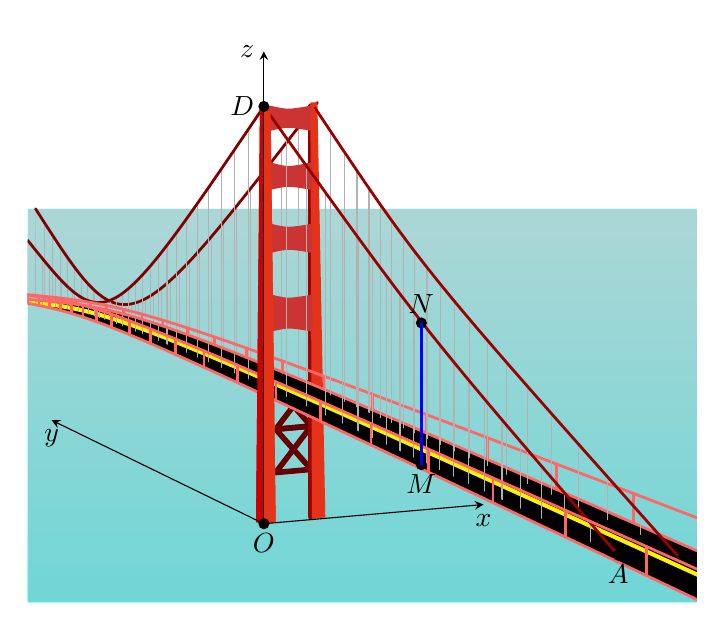
\begin{tikzpicture}[line join=round,line cap=round,>=stealth]
				 \clip (-3,-1) rectangle (5.5,6.3);
				\fill[opacity=0.8,bottom color= cyan!50!white,top  color= cyan!20!white] (-3,-1) rectangle (5.5,4);
				\begin{scope}
					\clip (0.68,5.35).. controls (-1.75,2.2)..  (-2.9,4) -- (-2.9,2.85).. controls (-2,2.5).. (0.68,1.75) -- (0.68,5.35);
					\foreach \i in  {1,2,...,30}
						{\path 
						(0.68,5.35).. controls (-1.75,2.2).. (-2.9,4) coordinate[pos=\i/30](x); 
					\draw[gray!60!white]  (x)--++(-90:4);}
				\end{scope}
				 \draw[red!50!black,line width=1pt] ((0.68,5.35).. controls (-1.75,2.2).. (-2.9,4);
				\draw[line width =2pt,red!40!black] (0.15,0.65)  -- (0.6,0.69) -- (0.15,1.2) -- (0.6,1.24) -- cycle;
				\draw[line width =2pt,red!40!black,shift={(0,0.55)}] (0.15,0.65)  -- (0.6,0.69) -- (0.15,1.2) -- (0.6,1.24) -- cycle;
				\draw[red!60!black,line width=2pt]  (0.59,0.09) -- (0.59,5.3);
				\fill[brown!40!red] 
					(0.61,0.06) -- (0.59,5.35) -- (0.68,5.35) -- (0.78,0.08) --  cycle;
				\fill[brown!40!red] (0,0) coordinate  (O) -- (0,5.3) coordinate (D) -- (0.085,5.3) -- (0.15,0.02) -- cycle;
				\fill[black!20!red] 
					(O) -- (D) -- (-0.05,5.32) -- (-0.1,0.02) --  cycle;
				\fill[brown!60!red,draw,gray!40!red,line width=0.5pt] (0.08,5.3).. controls (0.305,5.25).. (0.59,5.3) -- (0.591,5)..  controls (0.305,5.05)..(0.084,5) -- cycle;
				\fill[brown!60!red,draw,gray!40!red,line width=0.5pt] (0.085,4.58).. controls (0.306,4.52).. (0.603,4.58) -- (0.603,4.25).. controls (0.3065,4.3)..(0.086,4.25)  -- cycle;
				\fill[brown!60!red,draw,gray!40!red,line width=0.5pt] (0.091,3.8).. controls (0.307,3.75).. (0.605,3.8) -- (0.606,3.45).. controls (0.307,3.5)..(0.093,3.45) -- cycle; 
				\fill[brown!60!red,draw,gray!40!red,line width=0.5pt] (0.098,2.9)..  controls (0.308,2.85).. (0.608,2.9) -- (0.609,2.45).. controls (0.308,2.5)..(0.099,2.45) -- cycle;
				\fill (6,-1.2).. controls (-2,2.6)..  (-3,2.8) -- (-3,2.85).. controls (-1.5,2.72).. (7,-1)--cycle;
				\draw[yellow,line width = 1.5pt] (6.5,-1.1)..  controls (-1.75,2.66).. (-3,2.825);
				 \def\ipos{20}
				\begin{scope}
					\clip (0,5.3).. controls (-2,2.35).. (-3,3.6) -- (-3,2.8).. controls (-2.2,2.7)..  (0,1.75) -- cycle;
					\foreach \i  in {1,2,...,30}
						 {\path
						(0,5.3).. controls (-2,2.35).. (-3,3.6) coordinate[pos=\i/30](y); 
					\draw[gray!60!white] (y)--++(-90:4);} 
				\end{scope}
				 \draw[red!50!black,line width=1pt]
					 (0,5.3).. controls (-2,2.35).. (-3,3.6);
				\draw[line width=1pt,red!60!white] (7,-1).. controls (-1.5,2.72)..  (-3,2.85)
					(7,-0.5).. controls (-1.5,2.76).. (-3,2.91); 
				\foreach \t in {1,2,...,\ipos} 
					 {\path
					(7,-1) coordinate (c).. controls (-1.5,2.72).. (-3,2.85)  coordinate[pos=\t/\ipos](d)
					(7,-0.5) coordinate  (c').. controls (-1.5,2.76).. (-3,2.91) coordinate[pos=\t/\ipos](d');
				\draw[line width=1pt,red!60!white]  (d)--(d');}
				\begin{scope}
					\clip (D).. controls (2,2.5).. (4.5,-0.4) --  (0,1.75) --cycle;
					 \foreach \i in {1,2,...,20}
						 {\path
						(D).. controls  (2,2.5).. (4.5,-0.4) coordinate[pos=\i/20](x');
					\draw[gray!60!white]  (x')--++(-90:4);}
				\end{scope}
				\begin{scope}
					\clip (0.68,5.3).. controls (2,3.25).. (5.25,-0.35) -- (0.69,1.7) --cycle; 
					\foreach \i  in {1,2,...,20}
						{\path 
						(0.65,5.28).. controls (2,3.25)..  (5.25,-0.4) coordinate[pos=\i/20](y');
					\draw[gray!60!white]  (y')--++(-90:4);}
				\end{scope}
				\draw[red!60!black,line width=1pt] (D)..  controls (2,2.5).. (4.5,-0.4)
					(0.65,5.28).. controls (2,3.25)..  (5.25,-0.4);
				\draw[line width=1pt,red!60!white] (6,-1.2).. controls  (-2,2.6).. (-3,2.8)
					(6,-0.8).. controls (-2,2.78).. (-3,2.9); 
				 \foreach \t in {1,2,...,\ipos}
					{\path (6,-1.2) coordinate (a)..  controls (-2,2.6).. (-3,2.8) coordinate[pos=\t/\ipos](b)
					(6,-0.8) coordinate (a')..  controls (-2,2.78).. (-3,2.9) coordinate[pos=\t/\ipos](b');
				\draw[line  width=1pt,red!60!white] (b)--(b');}
				\fill[brown!40!red] (0,0) -- (0,5.3) -- (0.085,5.3) -- (0.15,0.02) -- cycle; 
				\fill[black!20!red] 
					(O) -- (D)  -- (-0.05,5.32) -- (-0.1,0.02) -- cycle;
				\fill (4.5,-0.4) coordinate (A) node[below]{$A$} circle  (2pt);
				\fill (2,0.75)  coordinate (M) node[below]{$M$} circle (2pt);
				\fill (2,2.55) coordinate  (N) node[above]{$N$} circle (2pt);
				 \draw[blue,line width=1pt] (M)--(N);
				\draw[->] (O) -- (154:3) node[below]{$y$}; 
				 \draw[->] (O) -- (5:2.8) node[below]{$x$};
				 \draw[->] (O) -- (90:6) node[left]{$z$};
				\fill  (O) node[below]{$O$} circle (2pt)
					(D)  node[left]{$D$} circle (2pt);
			\end{tikzpicture}
	\end{center}
	 \loigiai{
		\begin{center}
			\begin{tikzpicture}[line join=round,line cap=round,>=stealth]
					 \path
						(0,0) coordinate  (O)++(0:2) coordinate (x) node[below]{$x$}
						(O)++(90:4) coordinate  (D)++(90:1) coordinate (z) node[right]{$z$}
						(O)++(160:3)  coordinate (y) node[below]{$y$}
						(0,1)  coordinate (B)++(-20:4) coordinate (A)
						($(A)!.6!(D)$) coordinate  (N)
						($(A)!.6!(B)$) coordinate  (M)
						(O)++(-20:5) coordinate  (O');
					 \draw[->](O)--(x);
					\draw[->](O)--(y); 
					\draw[->](O)--(z); 
					\draw (B)--(A)--(D) 
						 (M)--(N)
						(O)--(O'); 
					\foreach \x/\y in{O/-90,A/-90,M/45,D/180,N/30}{\fill (\x) circle  (1pt)
						($(\x)+(\y:3mm)$) node {$\x$};} 
				\end{tikzpicture}
		\end{center}
		Chọn đơn vị  trên mỗi trục bằng $1$ m.\\
		 Ta có $A\in (Oyz)$ và $A$ cách mặt nước $75$ (m) và cách trục $Oz$ một khoảng $343$ (m) $\Rightarrow A(0;-343;75)$.\\
		Điểm $D$ là đỉnh cột trụ cách  mặt nước $227$ (m) $\Rightarrow \mathrm{d}(0;0;227)\Rightarrow \overrightarrow{AD}=(0;343;152)$.\\
		 Phương trình đường thẳng $AD$ là
		$\heva{& x=0 \\&  y=343t \\& z=227+152t}$, ($t \in\mathbb{R}$).\\
		Vì $N\in AD\Rightarrow  N(0;343t;227+152t)$.\\
		Điểm $M$ trên thành cầu, $M$ cách mặt nước $75$ (m) và cách trục $Oz$ một khoảng  bằng $230$ (m) nên tọa độ điểm $M$ là $M(0;-230;75)\Rightarrow \overrightarrow{MN} =(0;343t+230;152+152t)$.\\
		$MN$ song song với cột trụ $\Rightarrow MN \perp Oy \Rightarrow \overrightarrow{MN}\cdot\overrightarrow{j}=0 \Leftrightarrow  343t+230=0\Leftrightarrow t=-\dfrac{230}{343}$.\\
		$\Rightarrow  \overrightarrow{MN}=\left(0;0;\dfrac{17\,176}{343} \right)\Rightarrow MN=\dfrac{17\,176}{343}\approx 50{,}1$ (m).
	 }
\end{bt}

% nguồn: Phan2_Lop_12_Hinh_hoc_Chuong_5
\begin{bt}%[ma:6368662b]
	 %[2H5H1-6]
	Trong không gian $Oxyz$, góc giữa hai mặt phẳng $(P_1)\colon x+y+z-1=0$ và $(P_2)\colon x+2y-2z-3=0$~là $n^\circ$ (làm tròn kết quả đến hàng đơn~vị, $n$~là số nguyên dương). Giá trị của  $n$~là bao nhiêu?
	\shortans{79} 
	\loigiai{ 
		Ta có 
		\[\cos\left((P_1),(P_2)\right) =\dfrac{\left| 1\cdot 1+1\cdot 2+1\cdot (-2)\right|  }{\sqrt{1^2+1^2+1^2}\cdot \sqrt{1^2+2^2+(-2)^2}}=\dfrac{1}{\sqrt{3}}.\]
		Suy  ra $\left((P_1),(P_2)\right)\approx 79^\circ$. Vậy $n=79$.
	 }
\end{bt}

% nguồn: Phan2_Lop_12_Hinh_hoc_Chuong_5
\begin{bt}%[ma:a7d99148]
	%[2H5C3-4] 
	Một cơ sở sản xuất kem làm một mô hình Kem ốc quế lớn gồm $2$ phần: Phần Kem có dạng hình tròn $(C)$ là phần tiếp xúc giữa phần Kem và phần ốc quế. Chọn hệ  trục tọa độ $Oxyz$ trong không gian thoáng, phần Kem có hình cầu có tâm $I(1;2;3)$, bán kính $R_c = 3$ và phần đỉnh của hình nón là điểm $H(0;1;-2)$ đây là đường tròn có bán kính $R_N = \sqrt{6}$. Để tối ưu hóa lượng ánh sáng chiếu đèn có thể chiếu vào cây kem, người ta tính toán rằng chiếc đèn Led sẽ phải ở vị trí $M(a;b;2)$, $a \in Z$ và từ điểm $M$ kẻ được 2 tiếp tuyến với đường tròn $(C)$ sao cho góc giữa hai tiếp tuyến đó không bé hơn $60^\circ$.
	\begin{center}
		\resizebox{!}{5cm}{\begin{tikzpicture}[line join=round,line cap=round,>=stealth]
		\begin{scope}
			\path[ball color=yellow!60!green] (0,0) circle[radius=2cm]; 
			\coordinate (A) at  ($(0,0)+(-30:2cm)$);
			\fill  (A) circle (1pt);
			\coordinate (B) at ($(0,0)+(-150:2cm)$); 
			\fill  (B) circle (1pt);
			\fill  (0,0) circle (1pt);
		\draw (-30:2cm and 2cm) arc[start angle=-30,end angle=210,x radius=2cm,y radius=2cm];
	\draw[red,dashed] (-30:2cm) arc[start angle=-30,end angle=-150,radius=2cm];
\draw (B) arc[start angle=-180,end angle=0,x radius=1.74cm,y radius=0.3 cm];
\draw[dashed] (B) arc[start angle=180,end angle=0,x radius=1.74cm,y radius=0.3 cm];
\coordinate (M)  at ($(A)!0.5!(B)$);
\coordinate (I) at  ($(0,0)+(-90:5cm)$);
 \filldraw[ball color=orange]
	(B) arc[start angle=-180,end angle=0,x radius=1.74cm,y radius=0.3cm] --
	(A)  -- (I) -- cycle;
\draw  (A)--(I)--(B);
\end{scope}
\begin{scope}[shift={(6,0)}]
	\coordinate (A) at  ($(0,0)+(-30:2cm)$);
	\fill (A) circle  (1pt);
	\coordinate (B)  at ($(0,0)+(-150:2cm)$);
	\fill (B) circle  (1pt);
	\fill (0,0) circle (1pt) node[above] {$I$}; 
\draw (-30:2cm and 2cm) arc[start angle=-30,end angle=210,x radius=2cm,y radius=2cm];
\draw[blue,dashed] (-30:2cm) arc[start angle=-30,end angle=-150,radius=2cm];
\draw[dashed] (B) arc[start angle=180,end angle=0,x radius=1.74cm,y radius=0.3 cm];
\coordinate  (M) at ($(A)!0.5!(B)$);
\fill  (M) circle (1pt);
\coordinate (I) at  ($(0,0)+(-90:5cm)$);
\fill (I) circle (1pt)  node[right] {$H$};
\draw (B) arc[start angle=-180,end angle=0,x radius=1.74cm,y radius=0.3 cm];
 \draw (A)--(I)--(B);
\end{scope}
\end{tikzpicture}
		} 
	\end{center}
	\shortans{6} 
	\loigiai{ 
	\immini{Ta có $O I=\sqrt{R_C^2-R_N^2}=\sqrt{3^2-(\sqrt{6})^2}=\sqrt{3}$.\\ 
		$I H=\sqrt{(-1)^2+(-1)^2+(-5)^2}=3  \sqrt{3}$.\\
		$\dfrac{I O}{I H}=\dfrac{\sqrt{3}}{3 \sqrt{3}}=\dfrac{1}{3} \Rightarrow \overrightarrow{I O}=\dfrac{1}{3} \overrightarrow{I  H}$.\\
		Suy ra $$\heva{&x_0-1=-\dfrac{1}{3} \\&y_0-2=-\dfrac{1}{3} \\& z_0-3=-\dfrac{5}{3}} \Leftrightarrow \heva{&x_0=\dfrac{2}{3} \\& y_0=\dfrac{5}{3}  \\& z_0=\dfrac{4}{3}} \Rightarrow O\left(\dfrac{2}{3}; \dfrac{5}{3}; \dfrac{4}{3}\right).$$
		}{\begin{tikzpicture}[line join=round,line cap=round,>=stealth]
		\coordinate (A) at  ($(0,0)+(-30:2cm)$);
		 \fill (A) circle (1pt);
		 \coordinate (B) at ($(0,0)+(-150:2cm)$);
		 \fill (B) circle (1pt);
		 \fill (0,0) circle (1pt) node[above] {$I$};
	\draw (-30:2cm and 2cm) arc[start angle=-30,end angle=210,x radius=2cm,y radius=2cm];
\draw[dashed] (-30:2cm) arc[start angle=-30,end angle=-150,radius=2cm];
\draw[dashed] (B) arc[start angle=180,end angle=0,x radius=1.74cm,y radius=0.3 cm];
 \coordinate (M) at ($(A)!0.5!(B)$);
\fill (M)  circle (1pt);
\coordinate (M1)  at ($(M)+(180:5cm)$);
\fill (M1) circle (1pt) node[below] {$M$}; 
\coordinate  (I) at ($(0,0)+(-90:5cm)$);
 \fill (I) circle (1pt) node[right] {$H$};
\draw (B) arc[start angle=-180,end angle=0,x radius=1.74cm,y radius=0.3 cm];
\draw  (A)--(I)--(B);
\coordinate (A1) at  ($(M)+(140:1.75cm and 0.3cm)$);
\fill  (A1) circle (1pt) node[above] {$A$};
\coordinate (B1) at  ($(M)+(-110:1.75cm and 0.3cm)$);
\fill (B1) circle (1pt)  node[below] {$B$};
 \draw[dashed] (A1)--(M)--(B1)
	(0,0)--(I) 
	 (M)--(M1)
	(M)--(A); 
\draw  (B)--(M1)--(B1);
\fill (M) circle (1pt)  node[below right,yshift=0.12cm] {$O$};
\coordinate (E)  at ($(M1)!0.87!(A1)$);
\draw (M1)--(E); 
 \draw[dashed](A1)--(E);
\end{tikzpicture}
		} 
		Mặt phẳng $(MAB)$ đi qua điểm $O\left(\dfrac{2}{3};  \dfrac{5}{3}; \dfrac{4}{3}\right)$ và có VTPT $\vec{n} = \overrightarrow{HI} = (1;1;5)$
		Phương trình mặt phẳng  $(MAB)$
		$$1 \left( x - \dfrac{2}{3} \right) + 1 \left( y - \dfrac{5}{3} \right)  + 5 \left( z - \dfrac{4}{3} \right) = 0 \Rightarrow x + y + 5z - 9 = 0.$$
		Vì $M \in (MAB)$ nên $a  + b + 5.2 - 9 = 0 \Rightarrow a + b + 1 = 0 \Rightarrow b = -a - 1$.\\
		Khi đó $OM = \sqrt{\left( a - \dfrac{2}{3} \right)^2 + \left( b - \dfrac{5}{3} \right)^2 + \left( 2 -  \dfrac{4}{3} \right)^2 } = \sqrt{2a^2 + 4a + 8 }$.\\
		 Ta có
		\begin{eqnarray*}
			\widehat{AOM} &=& \dfrac{1}{2} \widehat{AOB} = \dfrac{1}{2} (180^\circ -  \widehat{AMB})\\
			&=& 90^\circ - \dfrac{1}{2} \widehat{AMB} \leq 90^\circ - 60^\circ  = 60^\circ
		\end{eqnarray*}
		Vì $0^\circ < \widehat{AOM} < 60^\circ$ nên $\cos 0^\circ > \cos \widehat{AOM} \geq \cos  60^\circ \Rightarrow \cos \widehat{AOM} \geq \dfrac{1}{2}$. \qquad(1)\\
		$\cos \widehat{AOM} = \dfrac{OA}{OM} = \dfrac{\sqrt{6}}{\sqrt{2a^2 +  4a + 8 }} = \dfrac{3}{\sqrt{a^2 + 2a + 4}}$. \qquad(2)\\
		Từ  $(1)$ và $(2)$ suy ra
		\begin{eqnarray*}
			& &\dfrac{1}{2} \leq \dfrac{3}{\sqrt{a^2  + 2a + 4}} < 1\\
			&\Rightarrow& \dfrac{1}{4} \leq \dfrac{3}{a^2  + 2a + 4} < 1\\
			 &\Rightarrow& 3a^2 + 2a + 4 \leq 12\\
			&\Rightarrow& a^2 + 2a  - 8 \leq 0\\
			&\Rightarrow& -4 \leq a \leq  2.
		\end{eqnarray*}
		Vì $a  \neq -1$ nên $a \in \{-4; -3; -2; 0; 1; 2\}$.
	 }
\end{bt}

% nguồn: Phan2_Lop_12_Hinh_hoc_Chuong_5
\begin{bt}%[ma:402d79c0]
	%[2H5V1-7] 
	\immini{Trong một bể hình lập phương cạnh $1$ m có chứa một ít nước. Người ta đặt đáy bể nghiêng so với mặt phẳng nằm ngang. Biết rằng, lúc đó mặt nước có dạng hình bình hành $ABCD$ và khoảng cách từ điểm $A$, $B$, $C$ đến đáy bể tương ứng là $40$ cm, $44$ cm, $48$ cm. Đáy bể nghiêng so với mặt phẳng nằm  ngang một góc bao~nhiêu độ (làm tròn kết quả đến hàng phần chục)?}
	{\begin{tikzpicture}[scale=0.9,line join=round,line cap=round,>=stealth]
		 \path
			 (0,0) coordinate (O)
			(-1,-1.5)  coordinate (B)
			(3,0) coordinate  (C)
			 ($(C)-(O)+(B)$) coordinate (D);
		\foreach \i/\j in {O/O',B/B',C/C',D/D'} \draw  ($(\i)+(0,3)$) coordinate (\j)
			($(\i)+(0,1)$) coordinate (\i  1);
		\path[fill=cyan!40]  (O1)--(B1)--(D1)--(C1);
		\path[fill=cyan!50]  (B1)--(B)--(D)--(D1)--cycle;
		\path[fill=cyan!50]  (D1)--(D)--(C)--(C1)--cycle;
		\draw (O')--(B')--(D')--(C')--(C)--(D)--(B)--(B') 
			(D)--(D') 
			(O')--(C'); 
		\draw[dashed] (O')--(O)--(B) 
			 (O)--(C);
		\path (B)--(D) node[pos=0.5,sloped,below]  {$1$ mm};
		 \path (C)--(D) node[pos=0.5,sloped,below] {$1$ mm};
		\path (C)--(C')  node[pos=0.5,sloped,below] {$1$ mm};
		\begin{scope}[xshift=6cm]
			\path 
				(0,0)  coordinate (O)
				(-1,-1.5)  coordinate (B)
				 (3,-0.5) coordinate (C)
				($(C)-(O)+(B)$) coordinate  (D);
			\foreach \i/\j in {O/O',B/B',C/C',D/D'} \draw ($(\i)+(0.5,3)$)  coordinate (\j);
			 \path
				($(O)!1/3!(O')$)  coordinate (O1)
				 ($(B)!1/3!(B')$) coordinate (B1)
				($(C)!3/5!(C')$) coordinate (C1) 
				 ($(D)!3/5!(D')$) coordinate (D1);
			\path[fill=cyan!40] (O1)--(B1)--(D1)--(C1); 
			\path[fill=cyan!50]  (B1)--(B)--(D)--(D1)--cycle;
			\path[fill=cyan!50]  (D1)--(D)--(C)--(C1)--cycle;
			\draw  (O')--(B')--(D')--(C')--(C)--(D)--(B)--(B')
				 (D)--(D')
				 (O')--(C');
			\draw[dashed]  (O')--(O)--(B)
				 (O)--(C);
			\path (B)--(D)  node[pos=0.5,sloped,below] {$1$ mm};
			\path  (C)--(D) node[pos=0.5,sloped,below] {$1$ mm};
			 \foreach \i/\j/\k in {O1/B/135,B1/A/135,C1/C/45,D1/D/135} \draw (\i) ++(\k:0.3) node {$\j$};
		\end{scope}
	\end{tikzpicture}
	} 
	\shortans{2,3} 
	 \loigiai{
		\begin{center}
			\begin{tikzpicture}[line join=round,line cap=round,>=stealth]
					\path 
						(0,0)  coordinate (O)
						(-1,-1.5) coordinate  (B)
						(3,-0.5) coordinate (C) 
						($(C)-(O)+(B)$) coordinate  (D);
					\foreach \i/\j in {O/O',B/B',C/C',D/D'} \draw  ($(\i)+(0.5,3)$) coordinate (\j);
					 \path
						($(O)!1/3!(O')$)  coordinate (O1)
						($(B)!1/3!(B')$)  coordinate (B1)
						($(C)!3/5!(C')$) coordinate (C1) 
						($(D)!3/5!(D')$) coordinate  (D1)
						($(D)!1.5!(D')$) coordinate  (z)
						($(D)!1.5!(B)$) coordinate  (y)
						 ($(D)!1.5!(C)$) coordinate (x);
					\path[fill=cyan!40]  (O1)--(B1)--(D1)--(C1);
					\path[fill=cyan!50] (B1)--(B)--(D)--(D1)--cycle; 
					\path[fill=cyan!50]  (D1)--(D)--(C)--(C1)--cycle;
					 \draw (O')--(B')--(D')--(C')--(C)--(D)--(B)--(B')
						 (D)--(D')
						 (O')--(C');
					\draw[dashed]  (O')--(O)--(B)
						 (O)--(C);
					 \path (B)--(D) node[pos=0.5,sloped,below] {$1$ mm};
					\path (C)--(D) node[pos=0.5,sloped,below] {$1$ mm}; 
					\path  ($(D)-(B)+(B1)$) coordinate (A');
					\foreach \i/\j/\k in {O1/B/135,B1/A/135,C1/C/45,D1/D/135} \draw (\i) ++(\k:0.3) node  {$\j$};
					\foreach \i/\j in  {D/x,D/y,D/z}\draw[-stealth] (\i)--(\j);
					 \foreach \i/\j in {x/45,y/90,z/180}\draw (\i) ++(\j:0.3) node {$\i$};
					\draw  (B1)--(A') node [right] {$A'$};
				\end{tikzpicture}
		\end{center}
		Chọn hệ trục tọa độ như hình vẽ. Suy ra  $A(0;1;0{,}4)$, $B(1;1;0{,}44)$, $C(1;0;0{,}48)$. Ta có
		 $$\overrightarrow{AB}=\overrightarrow{DC}\Rightarrow D(0;0;0{,}44)\Rightarrow AD=\dfrac{\sqrt{626}}{25}.$$
		Ta lại có $$AA'=\mathrm{d}(A,(Oxz))=1\Rightarrow \cos (AA',AD)=\dfrac{AA'}{AD}\Rightarrow (AA',AD)\approx 2{,}3^\circ.$$ 
		Vậy đáy bể nghiêng so với mặt phẳng nằm ngang một  góc gần bằng $2{,}3^\circ$.
	} 
\end{bt}

% nguồn: Phan2_Lop_12_Hinh_hoc_Chuong_5
\begin{bt}%[ma:ce1d8824]
	 %[2H5C3-4]
	 \immini{
	Hai quả bóng dạng hình cầu có kích thước khác nhau lần lượt đặt vào góc một căn nhà hình hộp chữ nhật sao cho quả bóng tiếp xúc với hai bức tường và nền nhà của căn nhà đó. Trên bề mặt  của mỗi quả bóng, tồn tại một điểm có khoảng cách đến hai bức tường quả bóng tiếp xúc và đến nền nhà lần lượt~là $2$; $3$; $1$. Tính tổng độ dài các đường kính của hai quả bóng đó.}{
	\resizebox{!}{5cm}{\begin{tikzpicture}
		 \def\a{5}
		\def\b{3} 
		 \def\c{4}
		\path 
			 (0:0) coordinate (O)
			(0:\a) coordinate (y) 
			(90:\c) coordinate (z) 
			(-30:\b)  coordinate (x)
			($(x)+(y)-(O)$) coordinate  (xy)
			($(O)!.9!(z)$) coordinate (z1) 
			($(x)+(z1)-(O)$) coordinate  (xz1)
			 ($(y)+(z1)-(O)$) coordinate (yz1)
			 (O)++(25:0.4*\a) coordinate (I);
		\path[name path=oy] (O)--(y); 
		 \draw[-stealth] (O)--(x) node[below]{$x$};
		 \draw[-stealth] (O)--(z) node[left]{$z$};
		\path[name path=dtron] (I) circle  (0.25*\c);
		\path[name intersections={of=dtron and oy,by={A,B}}]; 
		\fill[color = orange!30] (O)--(y)--(yz1)--(z1); 
		 \path[name path=dtron,ball color =red] (I) circle (0.25*\c);
		\fill[left color=cyan!50,right color=cyan!20,opacity=0.3] (O)--(x)--(xz1)--(z1); 
		 \draw (O)--(A)
			(x)--(xy)--(y); 
		 \draw[dashed] (A)--(B);
		\draw[-stealth] (B)--(y) node[below]{$y$}; 
	\end{tikzpicture}
	 }
	 }
	 \shortans{12}
	 \loigiai{
		Phương trình mặt cầu~là $(S)  \colon (x-a)^2 + (y-b)^2 + (z-c)^2 =a^2$.\\
		Gọi $M(x;y;z)  \in (S)$ sao cho
		$\mathrm{d} \left(M,  (Oxy) \right) =1$,
		$\mathrm{d} \left(M, (Oyz) \right)  =2$,
		$\mathrm{d} \left(M, (Oxz) \right) =3$ \\ 
		 $\Rightarrow M(2;3;1) \in (S)
		\Rightarrow \hoac{&a=3+  \sqrt{2} = r_1\\&a=3- \sqrt{2} = r_2.}$\\
		Suy ra $2r_1 + 2r_2  =12$.
	} 
\end{bt}

% nguồn: Phan2_Lop_12_Hinh_hoc_Chuong_5
\begin{bt}%[ma:0427edd7]
	%[2H5V3-4] 
	 Trong không gian $Oxyz$, cho mặt cầu $(S)\colon x^2+y^2+z^2+2x-4y-2z+\dfrac{9}{2}=0$ và hai điểm $A(0;2;0)$, $B(2;-6;-2)$. Điểm $M(a;b;c)$ thuộc $(S)$ thỏa mãn $\overrightarrow{MA}\cdot\overrightarrow{MB}$ có giá trị nhỏ nhất. Tổng $a+b+c$ bằng bao~nhiêu?
	 \shortans{1}
	\loigiai{ 
		Ta  có $(S)\colon x^2+y^2+z^2+2x-4y-2z+\dfrac{9}{2}=0\Leftrightarrow (S)\colon (x+1)^2+(y-2)^2+(z-1)^2=\dfrac{3}{2}$.\\
		 Mặt cầu $(S)$ có tâm $I(-1;2;1)$, bán kính $R=\dfrac{\sqrt{6}}{2}$.\\
		Vì $IA=\sqrt{2}>R$ và $IB=\sqrt{82}>R$ nên hai điểm $A$, $B$ nằm ngoài mặt cầu  $(S)$.\\
		Gọi $K$ là trung điểm đoạn thẳng  $AB$ thì $K(1;-2;-1)$ và $K$ nằm ngoài mặt cầu $(S)$.\\
		Ta có \begin{eqnarray*}
		\overrightarrow{MA}\cdot\overrightarrow{MB}&=&(\overrightarrow{MK}+\overrightarrow{KA})\cdot(\overrightarrow{MK}+\overrightarrow{KB})\\ 
		&=&MK^2+\overrightarrow{MK}.(\overrightarrow{KA}+\overrightarrow{KB})+\overrightarrow{KA}\cdot\overrightarrow{KB}\\ 
		 &=&MK^2-KA^2.
	\end{eqnarray*}
	Suy ra  $\overrightarrow{MA}\cdot\overrightarrow{MB}$ nhỏ nhất khi $MK^2$ nhỏ nhất, tức là $MK$ nhỏ nhất.\\
	 Đánh giá $IM+MK\ge IK\Rightarrow R+MK\ge IK\Rightarrow MK$ $\ge IK-R$.\\
	Suy ra $MK$ nhỏ nhất bằng $IK-R$, xảy ra khi $I$, $M$, $K$ thẳng hàng và $M$  nằm giữa hai điểm $I$, $K$.\\
	Như vậy $M$ là giao điểm của đoạn thẳng $IK$ và mặt  cầu $(S)$.\\
	Có $\overrightarrow{IK}=(2;-4;-2)$, $IK=\sqrt{2^2+(-4)^2+(-2)^2}=2\sqrt{6}=4R=4IM$.\\ 
	Suy ra $\overrightarrow{IK}=4\overrightarrow{IM}\Leftrightarrow \heva{&2=4(a+1)\\&-4=4(b-2)  \\&-2=4(c-1)}\Leftrightarrow \heva{&a=-\dfrac{1}{2}\\&b=1\\&c=\dfrac{1}{2}.}$\\
	Vậy $a+b+c=1$. 
} 
\end{bt}

% nguồn: Phan2_Lop_12_Hinh_hoc_Chuong_5
\begin{bt}%[ma:f1edfbac]
	%[2H5C2-8] 
	\immini{Có một chiếc lồng bằng sắt dạng hình hộp chữ nhật $ABCD. A'B'C'D'$ có $AB=2$ m, $AD=3$ m, $AA'=1$ m. Người thợ hàn muốn hàn một thanh sắt $MN$ nối hai đọan $AD$ và $BD'$ (Hình $11$). Tính chiều dài ngắn nhất của đoạn thanh sắt $MN$. Làm tròn kết quả đến hàng phần trăm của mét.}{\resizebox{!}{5cm}{\begin{tikzpicture}[line join=round,line cap=round]
		\def\a{3.5} 
		\path (0:0) coordinate  (A)
			++(0:\a) coordinate (B) 
			 ++(60:\a/2) coordinate (C)
			($(A)+(C)-(B)$) coordinate (D) 
			($(A)+(90:\a)$) coordinate  (A')
			($(B)+(90:\a)$)  coordinate (B')
			 ($(C)+(90:\a)$) coordinate (C')
			($(D)+(90:\a)$) coordinate  (D')
			($(A)!1/2!(D)$) coordinate  (M)
			 ($(B)!1/2!(D')$) coordinate (N);
		\draw[dashed] (C)--(D)--(A) 
			(D)--(D') 
			 (M)--(N)
			 (B)--(D');
		\draw  (C)--(C')
			(A)--(A') 
			(B)--(B') 
			(A)--(B)--(C) 
			 (A')--(B')--(C')--(D')--cycle;
		 \foreach \x/\g in {A/180,B/0,C/0,D/180,A'/180,B'/0,C'/0,D'/180,M/-60,N/20}
		\fill (\x) circle  (1pt) node[shift={(\g:10pt)}]{$\x$};
		\draw (\a/2,-\a/4)  node[above]{\text{ Hình} 11};
	\end{tikzpicture}
	 }}
	 \shortans{0,89}
	\loigiai{ 
		Chọn hệ trục toạ độ $Oxyz$ có gốc toạ độ $O$ trùng với $D$ và $A(3;0;0)$, $C(0;2;0)$, $D'(0;0;1)$, $B(3;2;0)$.\\ 
		Phương trình đường thẳng  $AD\colon\heva{&x=t \\ &y=0\\ &z=0}\quad(t \in \mathbb{R})$.\\
		Phương trình đường  thẳng $BD'\colon\heva{&x=3t' \\ &y=2t' \\ &z=1-t'} \quad\left(t' \in \mathbb{R}\right)$.\\
		Ta có $M\in AD\Rightarrow M\ (t;0;0)$ và $N\in BD' \Rightarrow  N\left(3t'; 2t'; 1-t'\right)$ nên $\overrightarrow{MN}=\left(3t'-t; 2t'; 1-t'\right)$.\\
		$MN$ ngắn nhất  khi và chi khi $\heva{& \overrightarrow{MN} \cdot \overrightarrow{AD}=0\\ & \overrightarrow{MN} \cdot \overrightarrow{BD'}=0} \Leftrightarrow \heva{& 3t'-t=0\\ & 14t'-3t=1} \Leftrightarrow \heva{& t=\dfrac{3}{5} \\ & t'=\dfrac{1}{5}.}$\\
		Vậy $MN=\dfrac{2\sqrt{5}}{5} \approx 0{,}89$ (m). 
	} 
\end{bt}

% nguồn: Phan2_Lop_12_Hinh_hoc_Chuong_5
\begin{bt}%[ma:472d6cda]
	 %[2H5H3-4]
	Trong không gian với  hệ trục tọa độ $Oxyz$, đài kiểm soát không lưu sân bay có tọa độ $O(0;0;0)$, mỗi đơn vị trên trục ứng với $1$ km. Máy bay bay trong phạm vi cách đài kiểm soát $417$ km sẽ hiển thị trên màn hình ra đa. Một máy bay đang ở vị trí $A(-688;-186;8)$ chuyển động theo đường thẳng $d$ có vec tơ chỉ phương là $\overrightarrow{u}=(91;75;0)$ và hướng về đài kiểm soát không lưu. Vị trí sớm nhất mà máy bay xuất hiện trên màn hình ra đa là $B(a;b;c)$. Tính $a+b+c$.
	 \shortans{-367}
	 \loigiai{
		Không gian mà ra đa có thể quan sát nằm  trong mặt cầu tâm $O$, bán kính $417$ km (mặt cầu $(S)$).\\
		Phương trình  mặt cầu $(S): x^2+y^2+z^2=417^2$.\\
		Phương trình đường thẳng $d$ là:  $\heva{& x=-688+91t\\&y=-185+75t\\&z=8 }$.\\
		Vị trí sớm nhất mà ra đa phát hiện máy quay là giao điểm của đường thẳng $d$ và mặt cầu $(S)$  xác định bởi
		$$(-688+91t)^2+(-185+75t)^2+8^2=417^2\Leftrightarrow \hoac{&t=3\\&t=8}$$ 
		\begin{itemize}
			 \item Với $t=3$ thì $x=-415$; $y=40$; $z=8$.
			\item  Với $t=8$ thì $x=40$; $y=415$; $z=8$.
		\end{itemize}
		Vậy có $2$ giao diểm là $B(-415;40;8)$ và $C(40;415;8)$.\\ 
		Khi đó $\overrightarrow{AB}=(273;225;0)\Rightarrow  AB\approx 353{,}77$.\\
		$\overrightarrow{AC}=(728;600;0)\Rightarrow AC=  943,39$.\\
		Vậy vị trí gần nhất mà ra đa có  thể quan sát là $B(-415;40;8)$. \\
	Suy ra $a+b+c=-367$. } 
\end{bt}

% nguồn: Phan2_Lop_12_Hinh_hoc_Chuong_5
\begin{bt}%[ma:210f77f6]
	%[2H5H2-7] 
	Trong không gian với hệ tọa~độ $Oxyz$, góc giữa hai đường thẳng  $\Delta\colon \dfrac{x-8}{1}=\dfrac{y-9}{1}=\dfrac{z}{5},$ $ \Delta'\colon \dfrac{x+2}{1}=\dfrac{y-4}{-1}=\dfrac{z-9}{3}$~là $n^{\circ}$ (làm tròn kết quả đến hàng đơn~vị, $n$~là số nguyên dương). Giá trị của $n$~là bao nhiêu?\shortans{29}
	 \loigiai{
		Đường thẳng  $\Delta\colon \dfrac{x-8}{1}=\dfrac{y-9}{1}=\dfrac{z}{5}$ có vectơ chỉ phương~là $\vec{a}=(1;1;5).$\\
		Đường thẳng $ \Delta'\colon \dfrac{x+2}{1}=\dfrac{y-4}{-1}=\dfrac{z-9}{3}$ có  vectơ chỉ phương~là $\vec{a}'=(1;-1;3).$\\
		Ta  có
		 $$
		\cos \left(\Delta, \Delta'\right)=\dfrac{|1 \cdot 1+1 \cdot(-1)+5 \cdot 3|}{\sqrt{1^{2}+1^{2}+5^{2}} \cdot  \sqrt{1^{2}+(-1)^{2}+3^{2}}}=\dfrac{15}{\sqrt{297}} \Rightarrow\left(\Delta, \Delta'\right) \approx 29^{\circ}.
		 $$
	} 
\end{bt}
